\section{Experiment and Analysis}

This section presents a series of experiments to validate the proposed method in terms of physical realism and performance scalability. We also perform a comparative analysis against existing common approximation methods to evaluate its applicability and advantages in real-world scenarios.

\subsection*{Validation of Physical Realism}

\subsubsection*{Objective}
To verify whether the proposed method can accurately simulate the floating, sinking, and rotational behaviors of rigid bodies in fluids, with a particular focus on the correctness of torque effects.

\subsubsection*{Setup}
\begin{itemize}
		\item \itemheader{Platform} Unity 2022.3.29f1, Windows 11, 13th Gen Intel(R) Core(TM) i9-13900HX @ 2.20GHz, 16GB RAM.
		\item \itemheader{Scene} A lightweight plank freely falls into a static water body.
		\item \itemheader{Physical Settings}
		\begin{itemize}
				\item Water density $\rho = 1.33$.
				\item Plank density is lower than water to ensure floating.
				\item Energy dissipation terms are disabled to purely observe buoyancy effects.
		\end{itemize}
		\item \itemheader{Sampling Density} 200 surface samples per surface area.
\end{itemize}

\subsubsection*{Measurement Metrics}
\begin{itemize}
		\item Variation of the plank's center of mass height over time.
		\item Variation of the plank's lowest point height over time.
		\item Variation of the pitch angle of the plank's main surface normal over time.
\end{itemize}

\subsubsection*{Results}

\begin{figure}[H]
	\centering
	\scalebox{1}{
		\begin{tikzpicture}
			\begin{axis}[
				width=5in, height=2in,
				enlargelimits=false,
				xlabel={time (seconds)},
				ylabel={meter},
				ymin=-2, ymax=5, ytick={-2,-1,...,5},
				axis y line*=left,
			]
				\addplot[black] coordinates { (0,0) (5,0) };
				\addplot[olive] table[x=t, y=com] {../Thesis/figures/simulation-record.dat};
				\label{plot:exp1-com}
				\addplot[blue] table[x=t, y=min] {../Thesis/figures/simulation-record.dat};
				\label{plot:exp1-lowest}
			\end{axis}
			\begin{axis}[
				width=5in, height=2in,
				enlargelimits=false,
				xtick=\empty,
				ylabel={degree},
				ymin=0, ymax=90, ytick={0,15,...,90},
				axis y line*=right,
				ylabel near ticks, yticklabel pos=right,
				legend style={at={(0.98,0.4)}, anchor=south east, legend columns=1}
			]
				\addlegendimage{/pgfplots/refstyle=plot:exp1-com}
				\addlegendentry{center-of-mass}
				\addlegendimage{/pgfplots/refstyle=plot:exp1-lowest}
				\addlegendentry{lowest point}
				\addplot[color=red] table[x=t, y=rx] {../Thesis/figures/simulation-record.dat};
				\addlegendentry{pitch}
			\end{axis}
		\end{tikzpicture}
	}
	\caption{Motion data gathered from real-time logs.}
	\label{fig:exp1}
\end{figure}

\subsubsection*{Analysis}

\begin{itemize}
		\item The plank quickly experiences localized buoyant forces upon contacting the water and starts rotating, eventually stabilizing with its large face facing upward.
		\item The center of mass height exhibits a typical damped oscillation, consistent with real-world floating behavior.
\end{itemize}

\subsubsection*{Summary}
The experimental results confirm that the proposed method can effectively simulate buoyancy and induced rotational behaviors, with dynamics aligning with physical expectations.

\subsection*{Performance and Scalability Test}

\subsubsection*{Objective}
To test how the method impacts performance (FPS) as the number of submerged objects increases, and to evaluate load capacity under different sampling densities.

\subsubsection*{Setup}
\begin{itemize}
		\item \textbf{Same platform and water environment}.
		\item \itemheader{Scene} Lightweight blocks are continuously generated and dropped at a fixed rate.
		\item \itemheader{Comparative Variables}
		\begin{itemize}
				\item With water (buoyancy simulation enabled) vs. without water (baseline FPS).
				\item Different surface sampling densities ($s$): 10, 20, 50, 100 per object per surface area.
		\end{itemize}
\end{itemize}

\subsubsection*{Measurement Metrics}
\begin{itemize}
		\item FPS versus number of submerged objects.
		\item (Optional) Average per-frame buoyancy computation time.
\end{itemize}

\subsubsection*{Results}

\begin{figure}[H]
	\centering
	\begin{tikzpicture}
		\begin{axis}[
			width=6in, height=4in,
			enlargelimits=false,
			xlabel={Number of objects},
			xmin=0, xmax=100,
			ymin=0, ymax=200,
			ylabel=FPS,
			legend style={at={(1,0)}, anchor=south east, legend columns=1}
		]
			\addplot[black] table[x index=0, y index=1, col sep=comma] {./figures/exp2/d0.log};
			\addlegendentry{simulation off}

			\addplot[red] table[x index=0, y index=1, col sep=comma] {./figures/exp2/d10.log};
			\addlegendentry{$s=10$}

			\addplot[blue] table[x index=0, y index=1, col sep=comma] {./figures/exp2/d20.log};
			\addlegendentry{$s=20$}

			\addplot[green] table[x index=0, y index=1, col sep=comma] {./figures/exp2/d50.log};
			\addlegendentry{$s=50$}

			\addplot[purple] table[x index=0, y index=1, col sep=comma] {./figures/exp2/d100.log};
			\addlegendentry{$s=100$}
		\end{axis}
	\end{tikzpicture}
	\caption{FPS data gathered from running simulations at different sampling densities.}
	\label{fig:exp2}
\end{figure}

\subsubsection*{Analysis}

\begin{itemize}
	\item FPS decreases linearly with the number of submerged objects.
	\item Under low sampling density (10 samples/m$^2$), real-time performance (above 60 FPS) is maintained with up to 30–50 objects;
		under moderate sampling densities (20–50 samples/m$^2$), the threshold is lowered to 15-20 objects.
\end{itemize}

\subsubsection*{Summary}
The method demonstrates good scalability for moderate numbers of objects and allows flexible trade-offs between accuracy and performance by adjusting sampling density.

\subsection*{Comparative Analysis}

\subsubsection*{Objective}

Traditional sphere pontoon methods typically require manual or semi-automatic configuration based on the specific geometry of each object. For rugged or highly anisotropic objects, insufficient or improperly placed pontoons can lead to poor buoyancy simulation results.  
This experiment aims to validate that the proposed Monte Carlo surface sampling method can universally adapt to various complex geometries based on true physical distributions without manual intervention.

\subsubsection*{Design}

For each test object, multiple configurations of sphere pontoons with varying numbers and layouts were set up, alongside a configuration using the proposed method for comparison. All objects were released from the air into a water body (Figure \ref{fig:exp3-setup}), and the motion was recorded using the same metrics as in Experiment 1.

Two test models with significantly different shape characteristics were selected:
\begin{itemize}
	\item Blender's default ``Suzanne'' monkey head model (approximately isotropic with a complex surface).
	\item A long wooden bat (highly anisotropic aspect ratio).
\end{itemize}

\begin{figure}[H]
	\centering
	\begin{subcaptionblock}{0.55\textwidth}
		\centering
		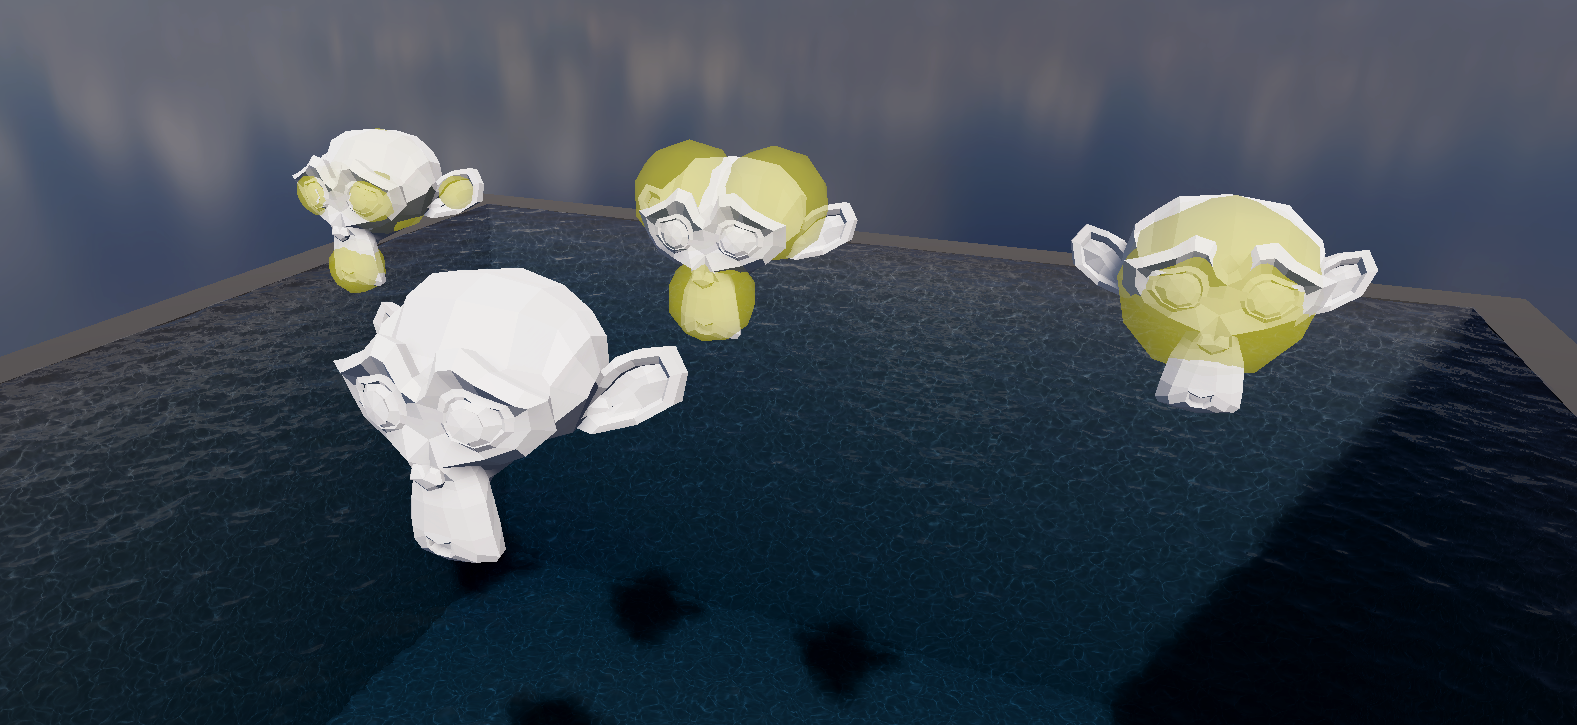
\includegraphics[height=1.3in]{./figures/exp3/suzzanes.png}
	\end{subcaptionblock}
	\begin{subcaptionblock}{0.4\textwidth}
		\centering
		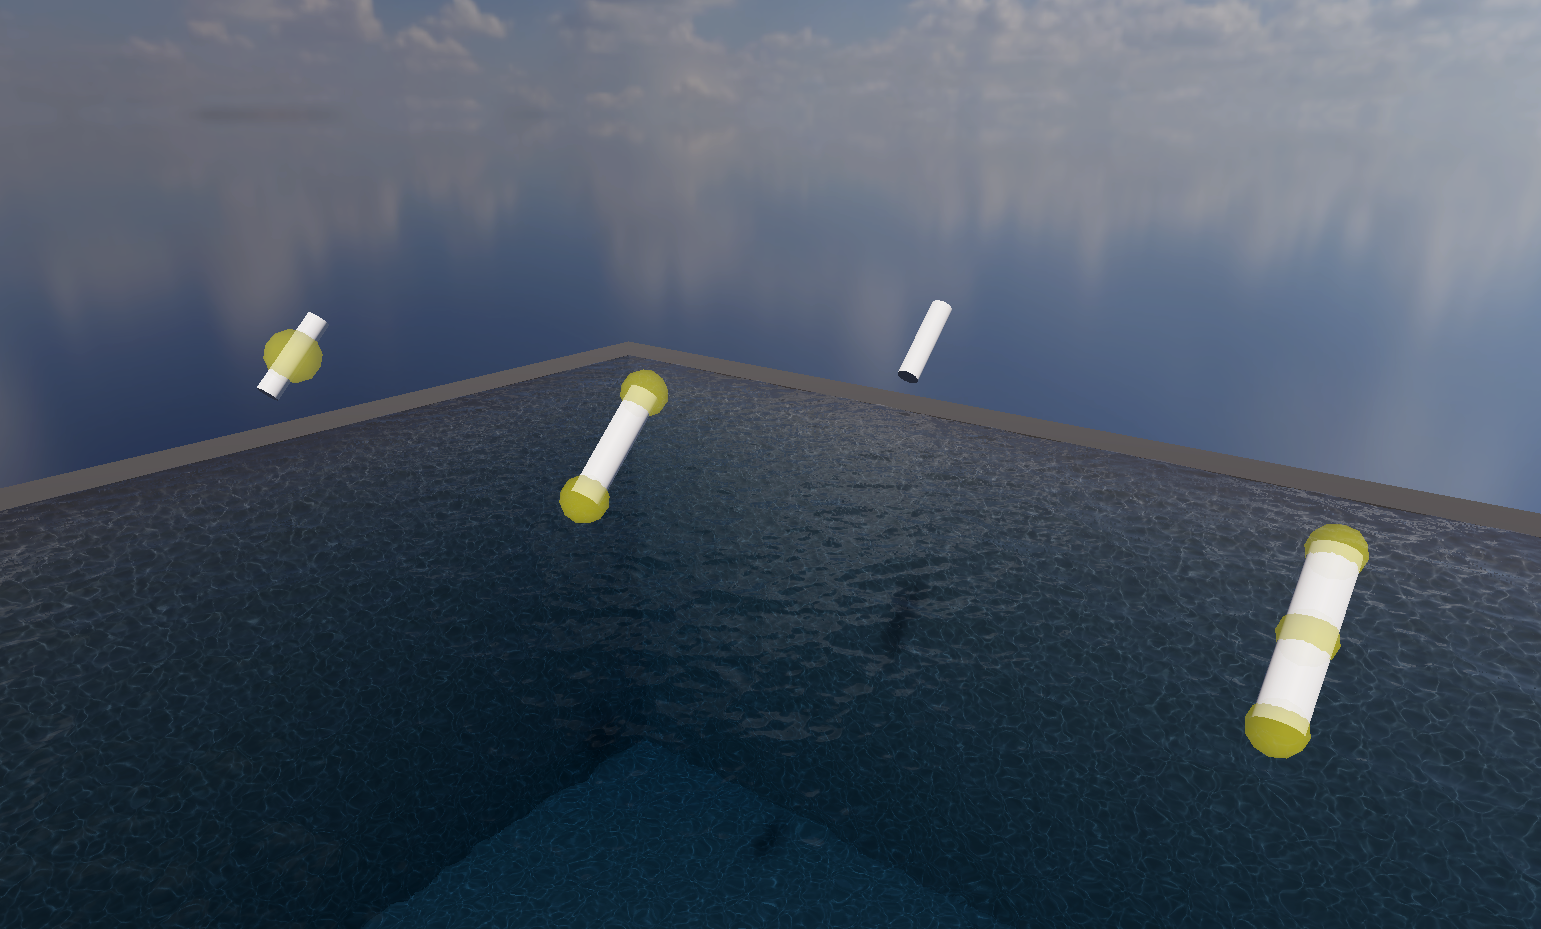
\includegraphics[height=1.3in]{./figures/exp3/bats.png}
	\end{subcaptionblock}
	\caption{The experiment setups.}
	\label{fig:exp3-setup}
\end{figure}

\subsubsection*{Results}

\begin{figure}[H]
	\centering
	\begin{tikzpicture}
		\def\plotsize{width=6in, height=4in, enlargelimits=false}

		% 高度
		\begin{axis}[
			\plotsize,
			xlabel={time (seconds)},
			xmin=0, xmax=5,
			ylabel={meter},
			ymin=-4, ymax=6,
			axis y line*=left,
		]
			\addplot[black,dashed] table[x=t, y=com] {./figures/exp3/suzzane/ours.log};
			\addplot[black,dotted] table[x=t, y=min] {./figures/exp3/suzzane/ours.log};

			\addplot[red,dashed] table[x=t, y=com] {./figures/exp3/suzzane/p1.log};
			\addplot[red,dotted] table[x=t, y=min] {./figures/exp3/suzzane/p1.log};

			\addplot[green,dashed] table[x=t, y=com] {./figures/exp3/suzzane/p3.log};
			\addplot[green,dotted] table[x=t, y=min] {./figures/exp3/suzzane/p3.log};
			
			\addplot[blue,dashed] table[x=t, y=com] {./figures/exp3/suzzane/p6.log};
			\addplot[blue,dotted] table[x=t, y=min] {./figures/exp3/suzzane/p6.log};
		\end{axis}

		\begin{axis}[
			\plotsize,
			xtick=\empty,
			xmin=0, xmax=5,
			ylabel={degree},
			ymin=270, ymax=360, ytick={270,285,...,360},
			axis y line*=right,
			ylabel near ticks, yticklabel pos=right,
			legend style={
				at={(1,1)},
				anchor=north east,
				nodes={scale=0.8},
			},
		]
			% 角度
			\def\rt{rx}
			\def\rsettings{forget plot}
			\addplot[\rsettings, color=black] table[x=t, y=\rt] {./figures/exp3/suzzane/ours.log};
			\addplot[\rsettings, color=red] table[x=t, y=\rt] {./figures/exp3/suzzane/p1.log};
			\addplot[\rsettings, color=blue] table[x=t, y=\rt] {./figures/exp3/suzzane/p3.log};
			\addplot[\rsettings, color=green] table[x=t, y=\rt] {./figures/exp3/suzzane/p6.log};

			% 图例

			% 第一列(线条类)
			\addlegendimage{black}
			\addlegendentry{pitch}

			\addlegendimage{black, dashed}
			\addlegendentry{center-of-mass}

			\addlegendimage{black, dotted}
			\addlegendentry{lowest point}

			\addlegendimage{white, opacity=0}
			\addlegendentry{}

			% 第二列(方块类)
			\addlegendimage{only marks, mark=square*, mark size=3pt, black}
			\addlegendentry{our method}

			\addlegendimage{only marks, mark=square*, mark size=3pt, red}
			\addlegendentry{1 pontoon}

			\addlegendimage{only marks, mark=square*, mark size=3pt, green}
			\addlegendentry{3 pontoons}

			\addlegendimage{only marks, mark=square*, mark size=3pt, blue}
			\addlegendentry{6 pontoons}
		\end{axis}
	\end{tikzpicture}
	\caption{Data collected from the Suzzane case.}
	\label{fig:exp3-suzzane}
\end{figure}

\begin{figure}[H]
	\centering
	\begin{tikzpicture}
		\def\plotsize{width=6in, height=2.5in, enlargelimits=false}

		% 高度
		\begin{axis}[
			\plotsize,
			xlabel={time (seconds)},
			xmin=0, xmax=5,
			ylabel={meter},
			ymin=-2, ymax=5,
			axis y line*=left,
		]
			\addplot[black,dashed] table[x=t, y=com] {./figures/exp3/bat/ours.log};
			\addplot[black,dotted] table[x=t, y=min] {./figures/exp3/bat/ours.log};

			\addplot[red,dashed] table[x=t, y=com] {./figures/exp3/bat/p1.log};
			\addplot[red,dotted] table[x=t, y=min] {./figures/exp3/bat/p1.log};

			\addplot[green,dashed] table[x=t, y=com] {./figures/exp3/bat/p2.log};
			\addplot[green,dotted] table[x=t, y=min] {./figures/exp3/bat/p2.log};
			
			\addplot[blue,dashed] table[x=t, y=com] {./figures/exp3/bat/p3.log};
			\addplot[blue,dotted] table[x=t, y=min] {./figures/exp3/bat/p3.log};
		\end{axis}

		\begin{axis}[
			\plotsize,
			xtick=\empty,
			xmin=0, xmax=5,
			ylabel={degree},
			ymin=40, ymax=90, ytick={40,45,60,...,90},
			axis y line*=right,
			ylabel near ticks, yticklabel pos=right,
			legend style={
				at={(1,1)},
				anchor=north east,
				nodes={scale=0.8},
			},
		]
			% 角度
			\def\rt{rx}
			\def\rsettings{forget plot}
			\addplot[\rsettings, color=black] table[x=t, y=\rt] {./figures/exp3/bat/ours.log};
			\addplot[\rsettings, color=red] table[x=t, y=\rt] {./figures/exp3/bat/p1.log};
			\addplot[\rsettings, color=blue] table[x=t, y=\rt] {./figures/exp3/bat/p2.log};
			\addplot[\rsettings, color=green] table[x=t, y=\rt] {./figures/exp3/bat/p3.log};

			% 图例

			% 第一列(线条类)
			\addlegendimage{black}
			\addlegendentry{pitch}

			\addlegendimage{black, dashed}
			\addlegendentry{center-of-mass}

			\addlegendimage{black, dotted}
			\addlegendentry{lowest point}

			\addlegendimage{white, opacity=0}
			\addlegendentry{}

			% 第二列(方块类)
			\addlegendimage{only marks, mark=square*, mark size=3pt, black}
			\addlegendentry{our method}

			\addlegendimage{only marks, mark=square*, mark size=3pt, red}
			\addlegendentry{1 pontoon}

			\addlegendimage{only marks, mark=square*, mark size=3pt, green}
			\addlegendentry{2 pontoons}

			\addlegendimage{only marks, mark=square*, mark size=3pt, blue}
			\addlegendentry{3 pontoons}
		\end{axis}
	\end{tikzpicture}
	\caption{Data collected from the wooden bat case.}
	\label{fig:exp3-bat}
\end{figure}

\subsubsection*{Analysis}

\begin{itemize}
	\item Under the same configuration of the water's physical properties, our method tends to create a softer response.
	\item Using the sphere pontoon method, deploying only one pontoon easily results in unnatural rotations (especially in the bat case, where using only one pontoon couldn't make the bat's pitch converge to zero). Achieving acceptable physical behavior requires increasing the number of pontoons and manually fine-tuning their positions and sizes.
	\item In contrast, our Monte-Carlo-based method requires no configuration. It directly estimates buoyancy and torque dynamically based on actual water-contact surfaces, achieving automatic adaptation and efficient simulation even for highly complex geometries.
\end{itemize}

\subsubsection*{Summary}

This experiment confirms that for objects of varying complexity and shape characteristics, traditional sphere pontoon methods heavily depend on the quantity and precision of configurations to accurately simulate buoyancy and torque.  
By comparison, the proposed method uses a unified, automated sampling workflow to adapt to diverse geometries without manual intervention, offering a balanced solution between simulation realism and development convenience.